\begin{frame}{Transformer Variants}
  \begin{itemize}
    \item[$\blacktriangleright$] \textbf{Encoder-only:} BERT, RoBERTa
    \item[$\blacktriangleright$] \textbf{Decoder-only:} GPT, LLaMA, Falcon
    \item[$\blacktriangleright$] \textbf{Encoder-Decoder:} T5, BART, mT5
  \end{itemize}
  \vspace{1em}
  \textbf{Modifications:}
  \begin{itemize}
    \item[$\blacktriangleright$] \textbf{Long-range:} Longformer, BigBird
    \item[$\blacktriangleright$] \textbf{Efficient:} Linformer, Performer
    \item[$\blacktriangleright$] \textbf{Sparse:} Sparse Transformer, Reformer
  \end{itemize}
\end{frame}

\begin{frame}{BERT -- Bidirectional Encoder}
  \begin{columns}
    \begin{column}{0.58\textwidth}
      \textbf{Key Ingredients of BERT:}
      \begin{itemize}
        \item \textbf{Pre-training Corpora:}
          \begin{itemize}
            \item English Wikipedia (\textasciitilde2.5B words)
            \item BookCorpus (\textasciitilde800M words)
          \end{itemize}
        \item \textbf{Pre-training Tasks:}
          \begin{itemize}
            \item \textbf{MLM} (Masked Language Modeling): Predict randomly masked words in context
            \item \textbf{NSP} (Next Sentence Prediction): Predict if two sentences naturally follow each other
          \end{itemize}
        \item \textbf{Model Sizes:}
          \begin{itemize}
            \item \textbf{BERT-Base:} 110M parameters
            \item \textbf{BERT-Large:} 340M parameters
          \end{itemize}
      \end{itemize}
    \end{column}
    \begin{column}{0.42\textwidth}
      \centering
      % BERT diagram or architecture image
      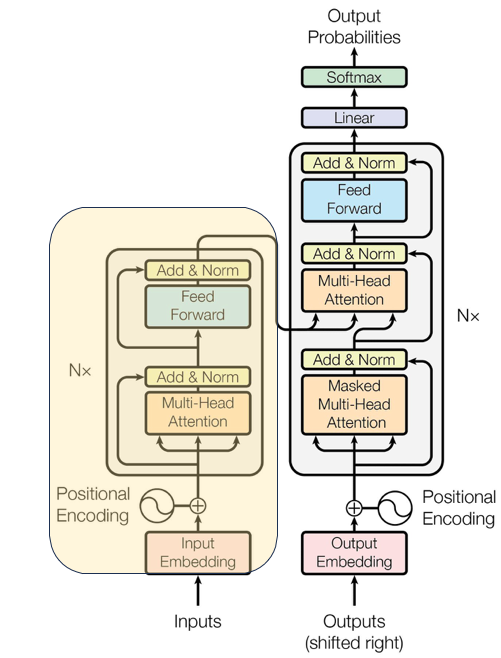
\includegraphics[width=0.98\textwidth]{assets/Lecture-6_Introduction_to_Transformers/pdf_page_091.png}
    \end{column}
  \end{columns}
\end{frame}

\begin{frame}{BERT -- Bidirectional Encoder}
  \begin{columns}
    \begin{column}{0.57\textwidth}
      \vspace{-0.2em}
      \textbf{What is our takeaway from BERT?}
      \begin{itemize}
        \item \textbf{Pre-training tasks can be invented flexibly\ldots}
          \begin{itemize}
            \item Effective representations can be derived from a flexible regime of pre-training tasks.
          \end{itemize}
        \item \textbf{Different NLP tasks seem to be highly transferable with each other\ldots}
          \begin{itemize}
            \item As long as we have effective representations, that forms a general model which can serve as the backbone for many specialized models.
          \end{itemize}
        \item[] \textcolor{red}{\textbf{And scaling works!!!}}
          \begin{itemize}
            \item[] {\color{red} 340M was considered large in 2018}
          \end{itemize}
      \end{itemize}
    \end{column}
    \begin{column}{0.43\textwidth}
      \centering
      % BERT architecture/diagram placeholder
      \vspace{-0.5em}
      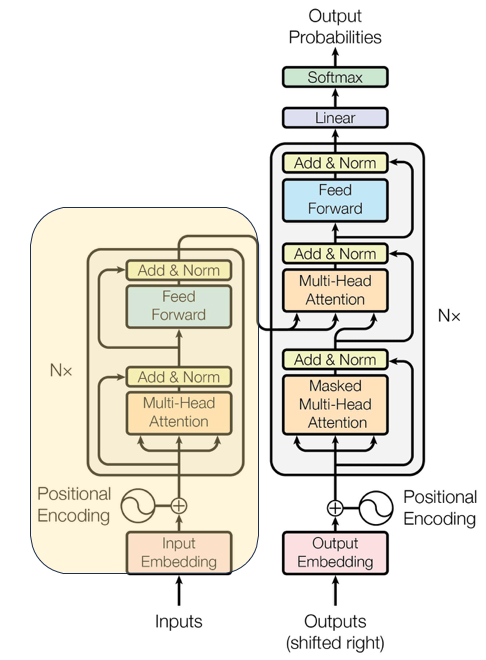
\includegraphics[width=\textwidth]{assets/Lecture-6_Introduction_to_Transformers/pdf_page_092.png}
    \end{column}
  \end{columns}
\end{frame}

\begin{frame}{GPT -- \textcolor{yellow}{\textbf{Generative}} Pretrained Transformer}
  \begin{columns}
    \begin{column}{0.60\textwidth}
      \textbf{GPT Pre-Training Corpus:}
      \begin{itemize}
        \item Similarly, BooksCorpus and English Wikipedia
      \end{itemize}
      \vspace{1.0em}
      \textbf{GPT Pre-Training Tasks:}
      \begin{itemize}
        \item Predict the next token, given the previous tokens
        \item More learning signals than MLM
      \end{itemize}
      \vspace{1.0em}
      \textbf{GPT Pre-Training Results:}
      \begin{itemize}
        \item GPT -- 117M Params
        \item Similarly competitive on GLUE and SQuAD
      \end{itemize}
    \end{column}
    \begin{column}{0.38\textwidth}
      \centering
      % Diagram: GPT architecture (placeholder)
      \vspace{0.5em}
      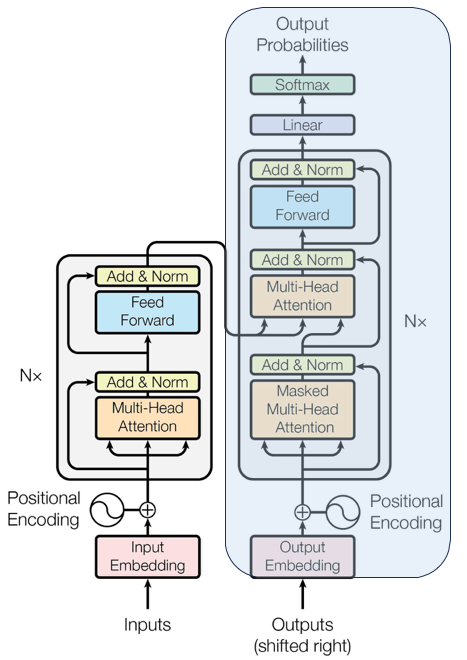
\includegraphics[width=0.98\textwidth]{assets/Lecture-6_Introduction_to_Transformers/pdf_page_093.png}
    \end{column}
  \end{columns}
\end{frame}

\begin{frame}{GPT -- \textcolor{yellow}{\textbf{Generative}} Pretrained Transformer}
  \begin{columns}
    \begin{column}{0.62\textwidth}
      \textbf{What is our takeaway from GPT?}
      \begin{itemize}
        \item \textbf{The Effectiveness of Self-Supervised Learning}
          \begin{itemize}
            \item Specifically, the model seems to be able to learn from generating the language \emph{itself}, rather than from any specific task we might cook up.
          \end{itemize}
        \item \textbf{Language Model as a Knowledge Base}
          \begin{itemize}
            \item Specifically, a generatively pretrained model seems to have a decent zero-shot performance on a range of NLP tasks.
          \end{itemize}
        \item[] \textcolor{red}{\textbf{And scaling works!!!}}
      \end{itemize}
    \end{column}
    \begin{column}{0.35\textwidth}
      \centering
      % GPT architecture/diagram placeholder
      \vspace{0.5em}
      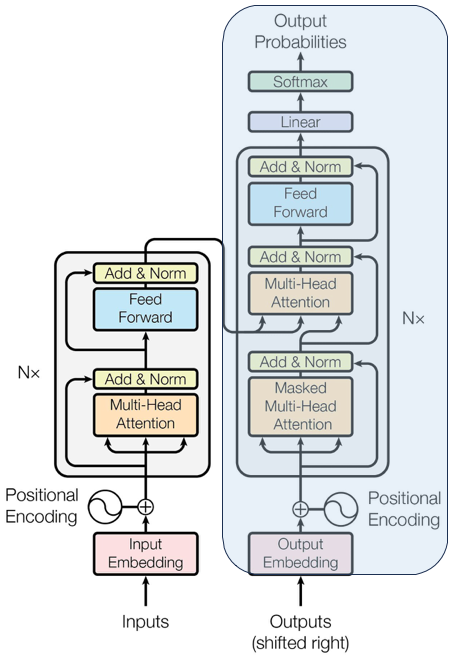
\includegraphics[width=\textwidth]{assets/Lecture-6_Introduction_to_Transformers/pdf_page_094.png}
    \end{column}
  \end{columns}
\end{frame}

\begin{frame}{The LLM Era -- Paradigm Shift in Machine Learning}
  \centering
  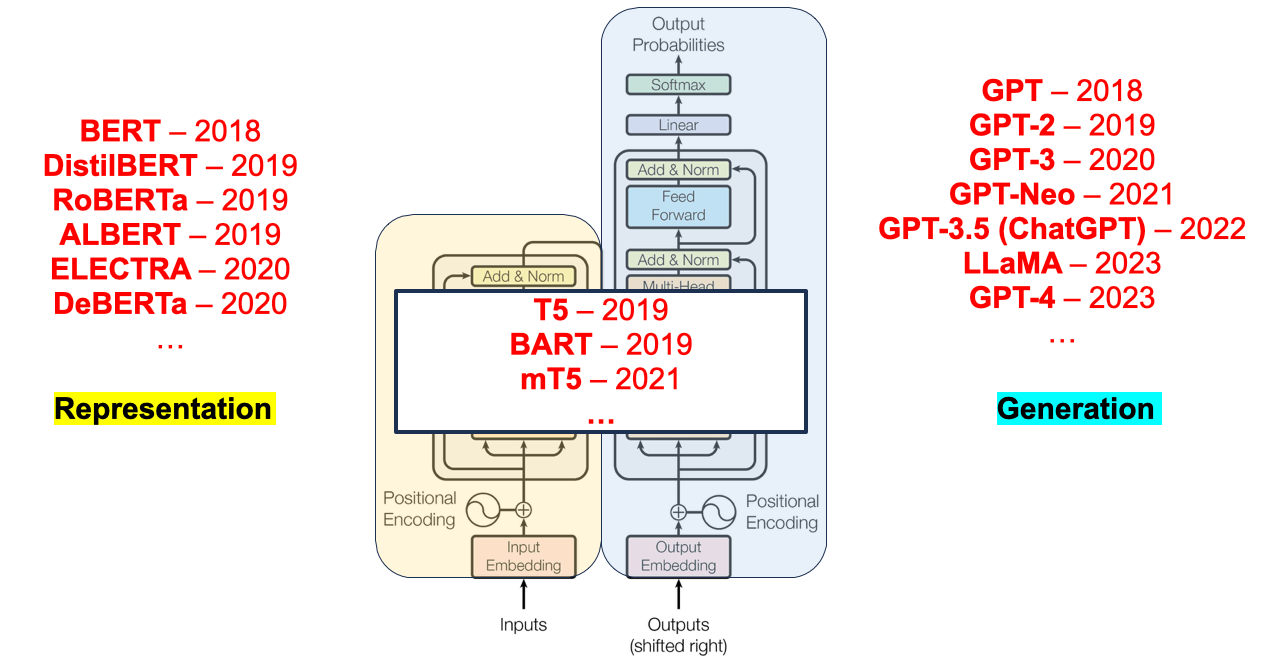
\includegraphics[width=0.8\paperwidth,height=0.8\paperheight,keepaspectratio]{assets/Lecture-6_Introduction_to_Transformers/pdf_page_095.png}
\end{frame}

